\section{Methods and Data}
\label{sec:ch3}

\subsection{Data Provenance}
\label{sec:ch3-data-provenance}

\subsubsection{WORKBank Database}
\label{sec:ch3-workbank}

The primary data source for this study is the WORKBank database, developed by Stanford University's SALT Lab as part of the "Future of Work with AI Agents" project (Shao et al., 2025). WORKBank represents a large-scale effort to understand human-AI collaboration potential across the occupational landscape, integrating multiple perspectives on task automation and augmentation requirements. The database was constructed through a large-scale data collection effort conducted in 2024-2025, capturing assessments from approximately 1,500 workers across 104 occupations and 52 domain experts evaluating 844 unique O*NET task descriptions.

By collecting paired assessments from both workers performing tasks and experts evaluating technical feasibility, WORKBank offers insight into the gaps between lived experience and technical capability. This dual-perspective approach can be particularly valuable for understanding intrapreneurial work, where tacit knowledge and contextual judgment play crucial roles.

All WORKBank assessments analyzed here pertain to tasks performed in the U.S. workforce.

\subsubsection{O*NET Task Descriptions}
\label{sec:ch3-onet}

O*NET (Occupational Information Network) provides the foundational task descriptions analyzed in this study. Sponsored by the U.S. Department of Labor's Employment and Training Administration, O*NET maintains extensive information on hundreds of standardized occupations, including detailed task statements that describe specific work activities performed within each occupation (Peterson et al., 2001). These task descriptions follow a standardized format and level of detail, supporting systematic analysis across diverse occupational contexts.

The O*NET Content Model structures occupational information hierarchically, with tasks representing the most granular level of work description. Each task statement describes a discrete, observable work activity using action verbs and specific objects or outcomes. For example: "Evaluate needs for procurement of funds and investment of surpluses and make appropriate recommendations" or "Design new or modify existing aerospace systems to reduce polluting emissions." This standardized structure supports consistent classification and analysis across a broad spectrum of occupational work.

For this study, we use the O*NET 30.0 Database. We utilize O*NET task statements, Importance and Frequency ratings, and the task-to–Work Activities and task-to-occupation (Standard Occupational Classification; SOC) link tables. Specifically:

\begin{itemize}
  \item \textbf{Importance and Frequency} are used to construct the Importance × Frequency (IF) quadrant framework that helps reveal where different types of work sit within occupational structures.
  \item \textbf{Work Activities (WA)} are used for downstream enrichment analysis (Section~\ref{sec:work-activities}; Appendix C.3, Table~\ref{tab:c3-work-activity}) and to derive autonomy-anchor features (e.g., \texttt{wa\_creative}, \texttt{wa\_strategic}; Appendix E.4, Table~\ref{tab:e4-autonomy-vars}).
  \item \textbf{Task metadata for LLM context}: minimal O*NET metadata (occupation title/SOC and associated Work Activities, when available) are supplied as task JSON context to the LLM classifier (Appendix~\ref{app:B}), in addition to the exact task text.
\end{itemize}

All O*NET joins are keyed by task\_id; SOC is used when merging occupation-level metadata. Outputs are consolidated into an analysis-ready task-level table (Appendix D.2, Table~\ref{tab:d2-data-paths}).

\textbf{Data limitations:} O*NET task descriptions, while comprehensive, are fundamentally bounded by standardization requirements. These statements average 15-20 words and emphasize observable activities, potentially underrepresenting cognitive and emotional dimensions of innovation work. Subtle intrapreneurial behaviors (informal influence, creative problem reframing, opportunity sensing) may appear less prominently in formal task taxonomies than in lived practice. Additionally, O*NET's static descriptions cannot fully capture temporal dynamics or the developmental progression from opportunity recognition through implementation. These limitations are inherent to any standardized occupational framework and should be considered when interpreting findings (see Section~\ref{sec:ch5-onet-limitations} for extended discussion).

\subsection{Samples and Scopes}
\label{sec:ch3-samples}

\subsubsection{Task-Level Samples}
\label{sec:ch3-task-level-samples}

Our analysis encompasses multiple overlapping samples reflecting different data availability and quality requirements:


\begin{itemize}
\item \textbf{IF-ready sample (N=844):} This deduplicated set of unique tasks contains complete O*NET Importance and Frequency ratings, enabling quadrant analysis. This serves as the core analytical sample for understanding the occupational positioning of intrapreneurial work. Six duplicate task entries were removed from legacy exports so that each task appears exactly once.

\item \textbf{HAS-complete subset (N=839):} This subset intersects the IF‑ready tasks with valid worker Human Agency Scale ratings and excludes the ambiguous case. Relative to the IF‑ready set (N=844), five tasks are dropped: the single ambiguous task; two tasks that lack worker HAS ratings (both non‑intrapreneurial); and two tasks with missing classification labels in the merged source used for downstream joins. This is the frame used for detailed human agency band analyses and worker–expert alignment; binary contrasts use 151 intrapreneurial and 688 non‑intrapreneurial tasks (total N=839).

\item \textbf{Intrapreneurial classification scope (N=844):} The label adjudication process covered all IF-ready tasks, yielding 153 classified as intrapreneurial (18.1\%), 690 as not intrapreneurial (81.8\%), and 1 as ambiguous (0.1\%). The ambiguous task is excluded from binary analyses but retained in the dataset for transparency.

\item \textbf{Sample count reconciliation (153 vs 151):} We report two closely related intrapreneurial counts depending on the analytical frame. The authoritative consensus set (844 unique tasks) contains 153 intrapreneurial tasks. Coverage‑filtered modules that require worker HAS operate on a task‑level frame (N=839), where intrapreneurial analyses use N=151 intrapreneurial tasks alongside 688 non‑intrapreneurial tasks. Relative to the IF‑ready classification frame (N=844), this reflects: dropping the single ambiguous task; excluding two tasks without worker HAS (both non‑intrapreneurial); and excluding two tasks with missing classification labels in the merged source used for downstream joins. We use 153 when referring to the main classification result and explicitly annotate N=151 in figures/tables derived from the coverage‑filtered frame.
\end{itemize}


\begin{table}[htbp]
\centering
\small
\caption{Sampling scopes and their usage}
\label{tab:scopes-usage}
\begin{tabular}{l r p{0.33\textwidth} p{0.33\textwidth}}
\toprule
Scope & N & Missingness Reason & Used In \\
\midrule
IF-ready sample & 844 & full sample with complete O*NET IF data & Section~\ref{sec:ch3-task-level-samples}; Section~\ref{sec:results} \\
HAS-complete subset & 839 & Drop 1 ambiguous; −2 tasks lack worker HAS (both non); −2 tasks have missing labels in merged source & Section~\ref{sec:human-agency} (HAS band analysis; alignment) \\
Classification scope & 844 & Same as IF-ready & Section~\ref{sec:ch3-label-adjudication}; Section~\ref{sec:results} \\
\bottomrule
\end{tabular}
\end{table}
  
Notes: All analyses use N=844 unless otherwise specified. Tasks with incomplete worker HAS assessments (two tasks) and the single ambiguous task are detailed in Appendix E (Table~\ref{tab:excluded-tasks}); Appendix E also lists two tasks excluded from coverage‑filtered joins due to missing classification labels in the merged source (Table~\ref{tab:excluded-missing-classification}). See Section~\ref{sec:results} for frame reconciliation.

\subsubsection{Occupation and Rater Coverage}
\label{sec:ch3-coverage}

The worker assessments span 104 distinct occupations selected to represent diverse skill levels, industry sectors, and task compositions. Occupations range from routine service roles to complex professional and managerial positions, providing broad coverage of the occupational landscape. Within each occupation, multiple workers provided ratings, with the number of raters per task tracked to assess response reliability.

Expert assessments were provided by 52 domain specialists with expertise in artificial intelligence, automation, and specific occupational domains. Unlike workers who rated only tasks within their own occupations, experts evaluated tasks across multiple occupations within their areas of expertise. This cross-occupational perspective allows experts to apply consistent technical standards while workers provide situated, experiential assessments.

\subsection{Label Adjudication Process}
\label{sec:ch3-label-adjudication}

\subsubsection{Theoretical Criteria Development}
\label{sec:ch3-criteria-dev}

The classification of intrapreneurial tasks employs six theory-grounded criteria derived from an extensive literature review (Neessen et al., 2018; Antoncic \& Hisrich, 2001; McMullen \& Shepherd, 2006; Alvarez \& Barney, 2007; Burgelman, 1983; Kuratko et al., 2005; Elliott et al., 2021):

\textbf{Criterion I – Opportunity Discovery and Idea Generation:} Tasks involving identification of unmet needs, market gaps, or process inefficiencies that present opportunities for value creation. Indicators include generating creative ideas, searching for new techniques, scanning environments for opportunities, and recognizing patterns others overlook.

\textbf{Criterion II – Planning, Preparation, and Advocacy:} Tasks focused on acquiring and orchestrating resources (financial, human, technological) often without formal authority. This encompasses developing business plans, building coalitions, acquiring sponsorship, and designing resource combinations.

\textbf{Criterion III - Execution, Implementation, and Active Behavior:} Tasks that implement new ideas and business activities. This includes putting effort into pursuing new business opportunities, managing the business through directing and decision-making, taking charge and exhibiting personal initiative, leading idea development and exploitation of new business activities, establishing new outlets or subsidiaries, launching new products or product–market combinations, recruiting/supervising/motivating employees, and finding solutions.

\textbf{Criterion IV - Innovative and Risk-Taking Behaviors:} Tasks that emphasize innovative, creative, or venturesome behavior. Indicators include showing innovative and creative behaviors, taking risks in the job, going for the "big win" when large interests are at stake despite potential downside, acting first and seeking approval later when appropriate, using out-of-the-box thinking, and voicing entrepreneurial ideas.

\textbf{Criterion V – Role-Specific Managerial Tasks:} Tasks involving formal or informal leadership in innovation contexts, differentiated by hierarchical level:
\begin{itemize}
  \item \textbf{V.A Senior-level:} Ratifying, recognizing, and directing roles; environmental scanning
  \item \textbf{V.B Middle-level:} Proposing, endorsing, refining, and shepherding opportunities
  \item \textbf{V.C First-level:} Experimenting, adjusting, and conforming processes
\end{itemize}

\textbf{Criterion VI – Eco-Innovation and Environmental Performance:} Tasks that explicitly involve environmental or sustainability objectives, such as:
\begin{itemize}
  \item Reducing material use during production (e.g., minimizing raw materials or waste).
  \item Reducing energy use during production (e.g., improving energy efficiency of processes or systems).
  \item Reducing emissions or other pollutants during production (e.g., lowering greenhouse gas or particulate emissions).
  \item Enabling environmental benefits during end-user consumption (e.g., designing products for recycling or reuse, developing systems that reduce environmental impact in use).
\end{itemize}

Intrapreneurship theory often highlights strategic renewal and business model innovation. In our operationalization, aspects of strategic renewal are captured indirectly when task descriptions involve new business activities, products, or processes under Criteria I–III, while Criterion VI focuses specifically on eco-innovation and environmental performance.


\begin{figure}[H]
\centering
% Robust include to avoid build break if image path varies across layouts
\IfFileExists{../03_Figures/Figure 3.1 Classification Flow from Criteria to Labels.png}{%
  \pandocbounded{\includegraphics[width=\textwidth,height=0.75\textheight,keepaspectratio]{../03_Figures/Figure 3.1 Classification Flow from Criteria to Labels.png}}%
}{\IfFileExists{../../Figure 3.1 Classification Flow from Criteria to Labels.png}{%
  \pandocbounded{\includegraphics[width=\textwidth,height=0.75\textheight,keepaspectratio]{../../Figure 3.1 Classification Flow from Criteria to Labels.png}}%
}{%
  \fbox{\parbox{0.9\textwidth}{Figure 3.1 image missing.}}
}}
\caption{Classification Flow from Criteria to Labels}
\label{fig:criteria-flow}
\end{figure}

The classification logic follows an inclusive-OR structure: a task qualifies as intrapreneurial if it satisfies any of the six criteria. This reflects the multi-dimensional nature of intrapreneurship theory. Tasks may exhibit opportunity discovery without strategic renewal, or managerial enabling without direct innovation execution. Tasks are classified as ambiguous only when the description provides insufficient evidence to confidently apply any criterion. Three independent classification runs with majority voting support label stability (see Section~\ref{sec:ch3-consensus}).

\textit{Clarification:} Although intrapreneurial execution often occurs under conditions of uncertainty and risk, the LLM prompt used for classification does not include a separate uncertainty keyword list. The classifier relies only on behavioral criteria (Criteria I–VI), emphasizing opportunity discovery, planning, execution of new business activities, innovative and risk-taking behaviors, and role-specific managerial and eco-innovation tasks. Uncertainty is measured independently through worker and expert ratings and the WBU index and is analyzed separately in the results; there we observe higher values for intrapreneurial work, rather than treating uncertainty as a direct classification rule.

The bullet-point definitions for Criteria I–VI in Section~\ref{sec:ch3-criteria-dev} mirror exactly the intrapreneurial criteria encoded in the LLM classification prompt (Appendix~\ref{app:B1}).

\subsubsection{Classification Procedure}
\label{sec:ch3-classification-procedure}

Each task underwent three independent classification runs using identical structured prompts encoding the theoretical criteria. The classification system was required to:

\begin{enumerate}
  \item Evaluate the task description against all six criteria and their sub-indicators.
  \item Document which specific criteria were satisfied and what textual evidence supported the classification.
  \item Assign a classification (Intrapreneurial/Not Intrapreneurial/Ambiguous) with confidence level.
  \item Provide structured justification linking the decision to theoretical foundations.
\end{enumerate}

All three runs used the same reasoning-capable large language model from OpenAI with identical prompts. Each run produced a complete record containing the classification decision, confidence score, matched criteria, and reasoning.

Consensus labels are obtained by aggregating the three runs through majority voting (Section~\ref{sec:ch3-consensus}).

\subsubsection{Consensus Through Majority Voting}
\label{sec:ch3-consensus}

The three classification runs were aggregated through majority voting to produce consensus labels. With three independent classifications per task:
\begin{itemize}
  \item \textbf{Unanimous agreement (777 tasks, 92.1\%):} All three runs produced identical classifications.
  \item \textbf{Majority agreement (67 tasks, 7.9\%):} Two runs agreed while one differed.
  \item \textbf{Ambiguous consensus (1 task, 0.1\%):} The task description was deemed insufficient for confident classification.
\end{itemize}

No ties occurred given the odd number of runs, and every task achieved at least majority consensus. The high unanimity rate suggests that the structured criteria help operationalize theoretical concepts into stable, reproducible decisions.

\subsection{Importance × Frequency (IF) Quadrant Construction}
\label{sec:ch3-if}

\subsubsection{Quadrant Framework}
\label{sec:ch3-quadrant-framework}

The Importance × Frequency (IF) quadrant framework divides the task landscape into four categories based on O*NET ratings:

\begin{description}
  \item[Core Quadrant:] High Importance (≥4.0) AND High Frequency (≥4.0) — the routine center of occupational practice.
  \item[Critical Quadrant:] High Importance (≥4.0) AND Low Frequency (<4.0) — episodic but consequential activities.
  \item[Operational Quadrant:] Low Importance (<4.0) AND High Frequency (≥4.0) — regular but peripheral activities.
  \item[Peripheral Quadrant:] Low Importance (<4.0) AND Low Frequency (<4.0) — margins of occupational practice.
\end{description}

The 4.0 thresholds for both dimensions represent analytical choices balancing interpretability with the observed distribution. O*NET's importance scale ranges from 1 (Not Important) to 5 (Extremely Important) with 4.0 corresponding to "Very Important." The frequency scale ranges from 1 (Yearly or less) to 7 (Hourly or more) with 4.0 approximating "More than weekly."

\textbf{Clarifying note on O*NET terminology:} O*NET also publishes “Core” versus “Supplemental” task flags based on (a) relevance (≥67\% of respondents) and (b) mean importance (≥3.0); tasks below these thresholds (or with <67\% relevance) are flagged as Supplemental. Those flags do not incorporate frequency and are conceptually distinct from our IF quadrants. Our use of “Core/Critical/Operational/Peripheral” names refers only to IF‑based quadrants and should not be conflated with O*NET’s Core/Supplemental task flags.

\subsubsection{Sensitivity Analysis}
\label{sec:ch3-sensitivity}

We repeated the quadrant assignment using three alternative threshold schemes in addition to the 4.0/4.0 baseline: a lenient specification (3.5/3.5), a strict specification (4.5/4.5), and a median split (Importance = 4.13, Frequency = 5.00). For each scheme, we reassigned quadrants, recomputed intrapreneurial prevalence by quadrant, and re-estimated enrichment odds ratios with FDR correction (Appendix C.1, Table~\ref{tab:c1-enrichment}). The core pattern of intrapreneurial depletion in the Core quadrant and enrichment in Critical and Peripheral quadrants remained qualitatively unchanged, with effect sizes attenuating under stricter thresholds. Worker–expert uncertainty gaps by quadrant showed similar stability across threshold choices (Appendix C.2, Table~\ref{tab:c2-uncertainty-gaps}). These results suggest that the positioning of intrapreneurial work in IF space is not solely an artifact of a particular cutoff choice.


\subsection{Human Agency Scale (HAS) Framework}
\label{sec:ch3-has}

\subsubsection{Scale Definition and Bands}
\label{sec:ch3-has-bands}

The Human Agency Scale, developed as part of the WORKBank project, characterizes the level
of human involvement required for effective task completion when AI assistance is available
(Shao et al., 2025). 

In the WORKBank survey, respondents rate this scale from their own perspective for each task; in this study we interpret these ratings as their preferred human–AI agency configuration for that task and use them both as descriptive measures and as inputs to the WBU index (Section~\ref{sec:ch3-uncertainty}). The scale comprises five levels:

\begin{itemize}
  \item \textbf{H1 (AI agent only / full automation):} 
        The AI agent takes primary responsibility for task execution and can handle the task entirely on its own without human involvement.

  \item \textbf{H2 (AI-led with human verification):} 
        The AI agent still drives task completion but needs human input or oversight at a few key points (e.g., checks, approvals, corrections).

  \item \textbf{H3 (Equal human–AI partnership):} 
        The human and the AI agent collaborate closely throughout the task; both contribute materially, and together they are expected to outperform either working alone.

  \item \textbf{H4 (Human-driven with AI assistance):} 
        The human takes primary responsibility for executing the task and remains in charge of outcomes, while the AI provides support or handles subtasks that still depend on human guidance and input.

  \item \textbf{H5 (Exclusively human):} 
        Task completion fully relies on human effort; AI does not provide meaningful assistance.
\end{itemize}

Both workers and experts rated each task on a 1–5 Human Agency scale. At the task level, we compute both (i) a mean HAS score (continuous) and (ii) a modal HAS band (H1–H5), defined as the most frequent integer response among raters. For workers, ratings are already discrete 1–5 and we take the mode directly. For experts, each HAS rating is first rounded to the nearest integer band (1–5) and then the mode is computed; ties are resolved in favor of the lower band. Analyses that treat agency as continuous use the mean HAS, whereas banded analyses (e.g., automation-proneness defined as H1/H2) use the modal HAS.

\subsubsection{Uncertainty Measures}
\label{sec:ch3-uncertainty}

Perceived task uncertainty was assessed via the WORKBank survey's ``Involved Uncertainty'' item, which asked respondents to rate ``the extent to which the task involves uncertainty or high-stakes decisions'' on a 1–5 scale. This measure captures both unpredictability and consequence, potentially conflating two constructs but providing insight into subjective risk perception. The \emph{Willingness to Bear Uncertainty (WBU)} index introduced below is our derived measure.

Preferences over automation were measured with the worker item:

\emph{``If an AI system can do this task for you completely, how much do you want an AI to do it for you?''}

Responses are recorded on a 1–5 Likert scale (1 = Not at all, 5 = Entirely) and referred to as \textit{AutomationDesire}.

To examine \textbf{willingness to bear uncertainty (WBU)}, we construct an index that combines uncertainty ratings with the gap between human agency preferences and automation desires:

\begin{equation}
\mathrm{WBU} = w(\text{uncertainty}) \times \big[ z_{\text{user}}(\text{HumanAgency}) - z_{\text{user}}(\text{AutomationDesire}) \big]
\end{equation}

with the uncertainty weight normalized to $[0,1]$:

\begin{equation}
w(\text{uncertainty}) = \frac{\text{involved\_uncertainty} - 1}{4}.
\end{equation}

Here, $z_{\text{user}}(\cdot)$ denotes within-user standardization of each rating to remove individual response-style differences. WBU is computed at the rating level and then aggregated to the task level (typically by taking the mean across workers for each task).

\subsection{Statistical Procedures}
\label{sec:ch3-stats}

\subsubsection{Enrichment Analysis}
\label{sec:ch3-enrichment}

To identify where intrapreneurial tasks concentrate within the IF quadrants, we employ Fisher's exact test comparing the proportion of intrapreneurial tasks in each quadrant to the baseline prevalence. Effect sizes are quantified through odds ratios (OR). For prevalence estimates, 95\% confidence intervals use Wilson score intervals. The same enrichment framework (OR via Fisher with FDR correction across the tested family) is used to identify over‑ and under‑represented O*NET Work Activities associated with intrapreneurial tasks (see Section~\ref{sec:work-activities}).

Multiple testing correction applies the Benjamini-Hochberg false discovery rate (FDR) procedure within test families. For the four quadrant comparisons, we report both raw p-values and FDR-adjusted q-values, using q<0.05 as the significance threshold.

\subsubsection{Paired Comparisons}
\label{sec:ch3-paired}

Worker-expert differences in uncertainty perceptions are analyzed using Wilcoxon signed-rank tests for paired samples. For each quadrant, we compute Δ = worker mean - expert mean at the task level, testing whether the median difference significantly differs from zero. Effect sizes are quantified through median differences with 95\% confidence intervals estimated via bootstrap (2000 iterations).

Within-quadrant correlations between worker and expert ratings employ Spearman's rank correlation coefficient (ρ) to assess monotonic associations robust to outliers. Bootstrap methods provide confidence intervals for correlation estimates.

\subsubsection{Categorical Associations}
\label{sec:ch3-categorical}

The distribution of HAS bands across intrapreneurial versus non-intrapreneurial tasks is compared using chi-square tests of independence. Cramér's V quantifies effect size for these categorical associations, with values interpreted as: small (0.1), medium (0.3), and large (0.5).

Agreement between worker and expert HAS band classifications is assessed through Cohen's kappa (κ), which corrects for chance agreement. Interpretation follows standard benchmarks: slight (0-0.20), fair (0.21-0.40), moderate (0.41-0.60), substantial (0.61-0.80), and almost perfect (0.81-1.00) agreement.

\subsubsection{Effect Size Reporting}
\label{sec:ch3-effect-sizes}

All statistical tests report appropriate effect sizes alongside significance tests:

\begin{itemize}
  \item \textbf{Odds ratios (OR):} For 2×2 enrichment analyses.
  \item \textbf{Spearman's rho (ρ):} For monotonic associations.
  \item \textbf{Cohen's kappa (κ):} For categorical agreement.
  \item \textbf{Cramér's V:} For multi-category associations.
\end{itemize}

Effect sizes provide scale-free measures enabling comparison across different analyses and assessment of practical significance beyond statistical significance.

\subsubsection{Importance–Frequency Correlation Analysis}
\label{sec:ch3-if-correlation}

To compare the coupling between O*NET Importance and Frequency across task types, we compute Spearman's rank correlation coefficient (\(\rho\)) separately for intrapreneurial tasks and their complement on the IF‑ready (IF‑only) sample. We assess the difference in correlations using Fisher's \(r\)-to‑\(z\) transformation with standard errors based on group sample sizes. Bootstrap (2000 iterations) provides confidence intervals for each \(\rho\). Summary results appear in Chapter~4 (Section~\ref{sec:results}), with the correlation table in Appendix C.4 (Table~\ref{tab:c4-if-correlation}).

\subsection{Ethics and Data Handling}
\label{sec:ch3-ethics}

\subsubsection{Ethical Considerations}
\label{sec:ch3-ethics-considerations}

The use of large language models for task classification raises considerations about algorithmic bias and transparency. To address these concerns, we provide complete classification criteria, document the prompt structure, and make consensus labels with justifications available for review.

\subsubsection{Data Quality and Integrity}
\label{sec:ch3-data-quality}

Multiple quality assurance procedures support data integrity:

\begin{itemize}
  \item \textbf{Deduplication:} Removal of duplicate task entries from legacy exports.
  \item \textbf{Completeness checks:} Verification that required fields contain valid values.
  \item \textbf{Response coverage:} Tracking number of raters per task to assess reliability.
  \item \textbf{Outlier detection:} Identification but retention of extreme values for transparency.
  \item \textbf{Missing data documentation:} Explicit reporting of sample sizes for each analysis.
\end{itemize}

When aggregating multiple ratings per task, we use means rather than medians to preserve information about the full response distribution. The number of unique raters is retained to enable weighting or filtering based on response coverage if desired.

\subsection{Reproducibility Provisions}
\label{sec:ch3-repro}

\subsubsection{Code and Documentation}
\label{sec:ch3-code-docs}

All analytical code is documented and organized by research question and analytical module. Analyses are implemented in Python 3.10+ using standard scientific computing libraries; visualization employs matplotlib and seaborn with consistent styling. Implementation details (scripts and exact data dependencies) are consolidated in Appendix D.1 (Key Scripts; Table~\ref{tab:d1-key-scripts}) and D.2 (Data Paths; Table~\ref{tab:d2-data-paths}). At a high level, the pipelines cover: label adjudication and voting; IF quadrant analysis; HAS profiling; uncertainty comparison (worker vs expert); and WBU computation.

\subsubsection{Data Availability}
\label{sec:ch3-data-availability}

Analytical datasets are structured to facilitate reproduction and extension:

- \textbf{Primary task dataset:} Contains task\_id, O*NET metadata, consensus labels, and justifications\\
- \textbf{Worker ratings:} Aggregated task-level means with rater counts\\
- \textbf{Expert ratings:} Aggregated task-level assessments \\
- \textbf{Quadrant assignments:} Task classifications under multiple threshold schemes

Data files use standard formats (CSV, Parquet) with documented schemas. Task identifiers enable joining across datasets for integrated analyses.

\subsubsection{Computational Environment}
\label{sec:ch3-env}

Analyses were implemented in Python 3.10+ using standard scientific libraries; full environment and requirements are documented in the accompanying code repository and Appendix D.

\subsection{Secondary Categorization of Intrapreneurial Tasks}
\label{sec:ch3-secondary}

\subsubsection{Rationale and Theoretical Grounding}
\label{sec:ch3-secondary-rationale}

To examine the internal composition of intrapreneurial work, we applied an additional, theory-guided categorization to tasks classified as intrapreneurial (153 in total), with descriptive analyses in Section~\ref{sec:results} based on the coverage‑filtered subset with complete metadata (N=151). This secondary analysis addresses whether the multi-dimensional nature of intrapreneurship identified in conceptual work (Antoncic \& Hisrich, 2001) manifests at the task level, which components dominate, and how they combine in practice.

\subsubsection{Category Framework}
\label{sec:ch3-category-framework}

The secondary analysis reorganizes and extends the primary classification criteria (Section~\ref{sec:ch3-criteria-dev}) for analytical purposes, allowing us to understand not just whether a task is intrapreneurial, but what type of intrapreneurial work it represents. While the primary criteria determine intrapreneurial classification through an inclusive-OR rule (any one criterion suffices), the secondary categories can co-occur within a single task to help characterize complex intrapreneurial patterns.

The relationship between primary classification criteria and secondary analytical categories is important to clarify. Categories I–IV in the secondary framework largely correspond to their counterparts in the primary criteria, maintaining consistency in opportunity discovery, planning, execution, and innovation dimensions. 

For the secondary analysis, we reconceptualize Category VI to focus on risk management and persistence aspects that emerge from the primary criteria’s emphasis on risk-taking behaviors (Criterion IV) and persistence/implementation aspects of primary Criterion III. The eco-innovation dimension from primary Criterion VI is incorporated within the innovation category (IV) when it appears in intrapreneurial tasks. 

In what follows, Roman numerals I–VI refer to secondary analytical categories; Category VI (Risk Management and Persistence) is a newly defined construct and is not the same as primary Criterion VI (Eco-Innovation and Environmental Performance). This reorganization better captures the operational realities of how intrapreneurial work manifests in practice.

We defined eight conceptual categories, implemented as five entrepreneurial components and three managerial subtypes. To maintain continuity with the primary criteria, the managerial subtypes retain the V.A/V.B/V.C notation, so the fifth entrepreneurial component is labeled VI rather than V.

Categories are non-mutually exclusive and draw on established intrapreneurship dimensions and process models:

\textbf{Entrepreneurial Core}
\begin{itemize}
  \item \textbf{I — Opportunity Discovery:} Scanning environments, recognizing patterns, identifying unmet needs or process inefficiencies. (Corresponds to primary Criterion I)
  \item \textbf{II — Planning, Preparation, and Advocacy:} Translating opportunities into plans, designs, or proposals; feasibility assessment; organizing action pathways; resource mobilization and internal issue selling. (Corresponds to primary Criterion II)
  \item \textbf{III — Action and Execution:} Implementing, deploying, or operationalizing new ideas; driving adoption and realizing outcomes. (Corresponds to primary Criterion III)
  \item \textbf{IV — Innovation and Experimentation:} Generating, recombining, or testing novel approaches; prototyping; creative problem-solving; includes eco-innovation when present. (Corresponds to primary Criterion IV, incorporates eco-innovation aspects from primary Criterion VI)
  \item \textbf{VI — Risk Management and Persistence:} Identifying and mitigating risks; ensuring quality/safety/compliance; persisting through obstacles; managing uncertainty. (Derived from risk-related aspects of primary Criterion IV and persistence/implementation aspects of primary Criterion III).
\end{itemize}

\textbf{Managerial Enablers (Burgelman, 1983; Kuratko et al., 2005):}
\begin{itemize}
  \item \textbf{V.A — Senior-level managerial actions:} Ratifying, recognizing, and directing roles; scanning the environment for opportunities and threats.
  \item \textbf{V.B — Middle-level managerial actions:} Proposing, endorsing, refining, and shepherding opportunities; identifying, acquiring, and deploying resources; linking groups.
  \item \textbf{V.C — First-level managerial actions:} Experimenting to surface operational improvements; adjusting processes through competence modification; conforming processes through competence deployment.
\end{itemize}

Inclusion of V.A/V.B/V.C managerial dimensions follows Zahra's argument that induced vs. autonomous forms and duration/context shape entrepreneurial outcomes (Zahra, 1993; Zahra \& Covin, 1995), which we map here to task-level enabling behaviors.

Categories I–II–III represent a process backbone (discovery → planning → execution). Category IV (innovation) cuts across stages as creative problem-solving. Category VI captures risk/quality concerns throughout. The three V.A/V.B/V.C categories reflect managerial roles that enable rather than replace entrepreneurial action.

Table~\ref{tab:criteria-category-mapping} clarifies the mapping between the primary classification criteria used to identify intrapreneurial tasks and the secondary analytical categories used to examine their internal composition.

\begin{table}[H]
\centering
\small
\caption{Mapping between primary classification criteria and secondary analytical categories}
\label{tab:criteria-category-mapping}
\begin{tabularx}{\textwidth}{l X X}
\toprule
Primary Criterion & Secondary Category & Notes on Transformation \\
\midrule
I - Opportunity Discovery and Idea Generation & I - Opportunity Discovery & Direct correspondence \\
II - Planning, Preparation, and Advocacy & II - Planning, Preparation, and Advocacy & Direct correspondence with consistent naming \\
III - Execution, Implementation, and Active Behavior & III - Action and Execution & Direct correspondence \\
IV - Innovative and Risk-Taking Behaviors & IV - Innovation and Experimentation \newline VI - Risk Management and Persistence (partial) & Innovation aspects map to Category IV; Risk-taking aspects contribute to Category VI \\
V - Role-Specific Managerial Tasks (V.A/V.B/V.C) & V.A - Senior-level managerial \newline V.B - Middle-level managerial \newline V.C - First-level managerial & Direct correspondence with sub-categories maintained \\
VI - Eco-Innovation and Environmental Performance & IV - Innovation and Experimentation (when eco-focused) & Eco-innovation incorporated within broader innovation category \\
\bottomrule
\end{tabularx}
\end{table}

\begin{table}[H]
\centering
\small
\caption{Illustrative examples of managerial subtypes (V.A/V.B/V.C)}
\label{tab:v-subtype-examples}
\begin{tabularx}{\textwidth}{l l X}
\toprule
Subtype & Occupation (task id) & Abridged task text \\
\midrule
V.A (Senior) & Computer and Information Systems Managers (970) & Stay abreast of advances in technology. \\
V.B (Middle) & Computer and Information Systems Managers (979) & Evaluate data processing proposals to assess project feasibility and requirements. \\
V.C (First) & Petroleum Engineers (3580) & Monitor production rates, and plan rework processes to improve production. \\
\bottomrule
\end{tabularx}
\end{table}

\subsubsection{Coding Procedure}
\label{sec:ch3-coding-procedure}

Category assignments are LLM-derived at the level of the primary criteria. During the primary classification runs (Appendix~\ref{app:B1}), the model outputs a \texttt{matched\_categories} field for each task indicating which primary Criteria I–VI and managerial subtypes V.A/V.B/V.C apply. 

For the secondary analysis, we construct the analytical categories described in Section~\ref{sec:ch3-category-framework} from these tags: I, II, and III map directly; innovation and eco-innovation tags (IV and primary VI) are combined into Category IV; and Category VI (Risk Management and Persistence) is derived from risk-related aspects of Criterion IV and persistence/implementation aspects of Criterion III. We apply this mapping to all intrapreneurial tasks (N=153; coverage-filtered N=151). Tasks can receive multiple category labels. Downstream scripts for the intrapreneurial composition analysis (internal “Q10” modules in the code base) parse the derived categories to compute prevalences, associations, and phenotypes.

\subsubsection{Phenotype Derivation}
\label{sec:ch3-phenotype-derivation}

From category combinations, we derived six task-level phenotypes via explicit truth tables. Table~\ref{tab:phenotype-derivation} summarizes the definitions.

\begin{table}[H]
\centering
\small
\caption{Phenotype derivation from category combinations}
\label{tab:phenotype-derivation}
\begin{tabular}{l l}
\toprule
\textbf{Phenotype} & \textbf{Definition} \\
\midrule
\textbf{FULL (Full-cycle)} & I + II + III (complete discovery-to-execution) \\
\textbf{DISC (Discovery-focused)} & I present, not FULL \\
\textbf{PLAN (Planning-focused)} & II present without I, not FULL \\
\textbf{EXEC (Execution-focused)} & III present without I or II \\
\textbf{INNOV (Innovation-focused)} & IV present, not FULL \\
\textbf{MGR (Managerial)} & Any V.* present \\
\bottomrule
\end{tabular}
\end{table}

Phenotypes are non-mutually exclusive; a task can be both INNOV and MGR, for example.

\subsubsection{Statistical Analysis}
\label{sec:ch3-secondary-stats}

We computed:
\begin{itemize}
  \item \textbf{Category prevalence:} Proportion of intrapreneurial tasks in the coverage‑filtered subset (N=151) containing each category.
  \item \textbf{Pairwise associations:} Fisher's exact tests with FDR correction to identify over- and under-represented category combinations.
  \item \textbf{Phenotype distribution:} Prevalence of each phenotype with 95\% confidence intervals.
  \item \textbf{Phenotype overlap:} Co-occurrence patterns among phenotypes.
\end{itemize}

Full technical details and association matrices are provided in Appendix F; truth tables are referenced therein.
